\documentclass[12pt,final]{article}

\title{Predicting Future Changes in a Publicly Traded Stock Using Historical Data and Methods from Probability}
\author{Rayhan Noufal Arayilakath\\ IB Mathematics Analysis and Approaches HL\\ Westlake Academy}
\date{2023\\ March}

\usepackage{graphicx}
\usepackage{mathtools}
\usepackage{float}
\usepackage{multirow}
\usepackage{blindtext}

\usepackage{xcolor}
\usepackage{listings}

\definecolor{dkgreen}{rgb}{0,0.6,0}
\definecolor{gray}{rgb}{0.5,0.5,0.5}
\definecolor{mauve}{rgb}{0.58,0,0.82}

\lstdefinelanguage{JavaScript}{
  keywords={typeof, new, true, false, catch, function, return, null, catch, switch, var, if, in, while, do, else, case, break},
  ndkeywords={class, export, boolean, throw, implements, import, this},
  comment=[l]{//},
  morecomment=[s]{/*}{*/},
  morestring=[b]',
  morestring=[b]",
  aboveskip=3mm,
  belowskip=3mm,
  showstringspaces=false,
  columns=flexible,
  basicstyle={\small\ttfamily},
  numbers=none,
  numberstyle=\tiny\color{gray},
  keywordstyle=\color{blue},
  commentstyle=\color{dkgreen},
  stringstyle=\color{mauve},
  breaklines=true,
  breakatwhitespace=true,
  tabsize=2
}

\lstset{
   language=JavaScript,
   extendedchars=true,
   basicstyle=\footnotesize\ttfamily,
   showstringspaces=false,
   showspaces=false,
   numbers=left,
   numberstyle=\footnotesize,
   numbersep=9pt,
   tabsize=2,
   breaklines=true,
   showtabs=false,
   captionpos=b
}

\setcounter{MaxMatrixCols}{20}

\newcommand*\mean[1]{\bar{#1}}

\begin{document}

\maketitle

\begin{abstract}
In this paper, I employ Markov Chains on a frequency distribution of historical three-day trading
statistics to calculate future statistics for a publicly traded stock and use said statistics to
predict possible changes, thus enabling me to plan for possible gains or losses from an investment 
and make profitable financial decisions.
\end{abstract}

\section{Introduction}
Recently I have been urged to start investing and maintaining a stock portfolio to make some
passive income throughout the school year, a time during which I cannot make a time commitment
to any job or internship. Since my interests are focused on the natural sciences and
technology, not particularly economic sciences, I initially started investing in stocks with
very little knowledge of how to work the markets to make a profit. I currently sit on a loss
amounting to quite a large sum (for an adolescent with no fixed income). After a few hits and
losses I gained a little experience and some better judgment, however, I wanted to have some
tools to earn back better and turn a profit on my investments. Most tools that I found were
paywalled and require more money than they are worth. This is a major blocker in my
quest to make some money. To solve this problem, I set out on building my tools and
creating my predictive model of stock futures to enhance my investments.

\section{Background}
With some experience in software development and data sciences, I approached this new project
with particular interest. I have used machine learning models in the past however I never took
care to examine the inner workings. I was aware of a technique in natural-language processing
that involves analyzing a linear sequence of words (a sentence) and through the usage of "Markov
Chains" generate text in a specific style based on a large corpus of text. Being a consumer, I
never explored the construction of Markov Chains, however, with some research, I found that Markov
Chains had a mathematical basis. In the field of Statistics, a Markov Chain is the
result of a modeling process that follows the Markov Property, such that the probability of the next
state in a sequence depends only on the current state. Mathematically this is represented in
the equation below:

\begin{equation}
  P(X_n=s_n|X_0=s_0,X_1=s_1,\dots,X_{n-1}=s_{n-1}) = P(X_n=s_n | X_{n-1}=s_{n-1})
  \label{eq:markovproperty}
\end{equation}

Where $X$ is some random variable that has a value from the state space $s$ and $n$ is the
time-step parameter. Here we dictate that the probability that the next state $X_n$ of some state
in $s_n$, given all the prior states, is the same as the probability that the next state $X_n$ of
some state in $s_n$ given only the current state $X_{n-1}$. A simple example of a state space
would be a coin toss, which has a state space of $s=\{Heads, Tails\}$ where each item in the
state space is a possible state or outcome of flipping a coin. At any given time-step $n$, the
probability of transitioning to a different state is 0.5 (as observed in typical coin-toss
behavior). If our state space ($s$) is finite (as in this coin example) and we use discrete
time-steps ($n$), we can apply the Markov Property to get the aforementioned Markov Chain from
the data. One can also apply the Markov Property to indiscrete time steps and variable state
spaces, although that is beyond the scope of understanding needed for this paper. Visually, the
Markov Chain for our example situation can be represented using the diagram seen in
Figure 1.

\begin{figure}[H]
  \begin{center}
    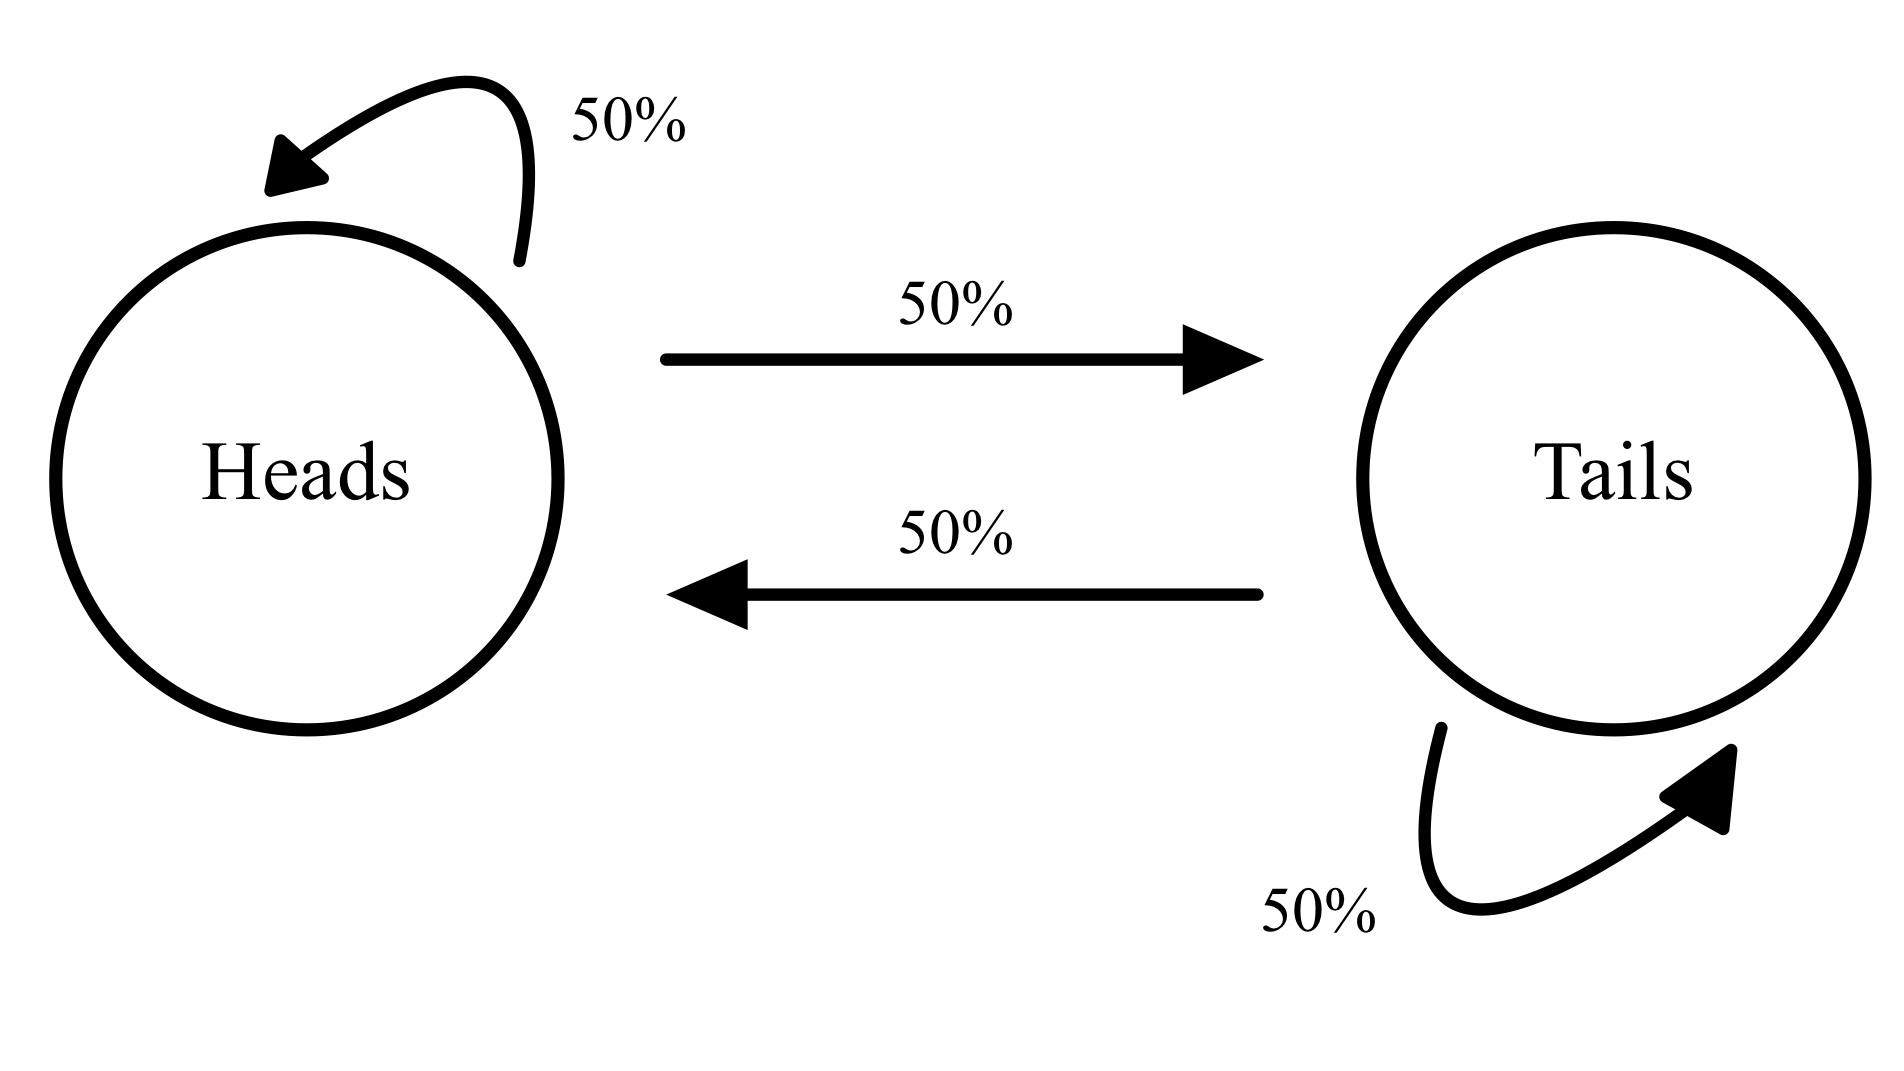
\includegraphics[width=0.95\textwidth]{figures/Figure-1}
  \end{center}
  \caption{A diagram representing the possible probabilities of moving from one state to another in the context of a coin toss. Created by the author in Notability.}
  \label{fig:markovchainexamplecointoss}
\end{figure}

The large nodes are the states from the state space $s$ and the percentages on the arrows
signify the probability of transitioning, best defined as the probability of moving from one state
to another. As one can see there is a probability of 0.5 of moving to a state of Tails starting at
Heads and there is a probability of 0.5 of moving to a state of Heads again. This is similarly
represented by movements from Tails. Mathematically, we can represent this data as a matrix of
transition probabilities, which is a type of matrix of $N$ by $N$ size, such that $N$ is the
number of items in the state space $s$ and the sum of the indices of each row or column, depending
on the direction of the matrix, add up to 1 (the matrix is stochastic). The transition matrix can
be used in the Markov Property as represented in the next equation:

\begin{equation}
  P_{i,j} = P(X_n=j | X_{n-1} = i) = P(X_n=s_n | X_{n-1}=s_{n-1})
  \label{eq:markovpropertywithtransitionmatrix}
\end{equation}

Where $i$ dictates the state you are currently at and $j$ dictates the state you will be at on the
next step. For our coin toss example, we would have the transition probability matrix $P$
seen below:

\begin{equation}
  P_{i,j}=\begin{bmatrix}
    0.5 & 0.5 \\
    0.5 & 0.5
  \end{bmatrix}
  \label{eq:transitionprobabilitymatrixcointoss}
\end{equation}

Where $i$ is aligned at the top with the columns and $j$ is aligned along the left with the rows.
The entry at index $(0,0)$ tells us that going from a state of Heads to Heads has a probability
of 0.5; similarly, the entry at index $(0,1)$ tells us that going from a state of Heads to Tails
has a probability of 0.5. The transition matrix also has another use - it can be integrated into
the Markov Equation to generate states for the Markov Chain. The Markov Equation (below) takes
the transition probability matrix and multiplies it by a state vector to output the probabilities
of the next state occurring.

\begin{subequations}
\begin{align}
  X_n = PX_{n-1} \\
  X_n = X_{n-1}P
\end{align}
\label{eq:markovequation}
\end{subequations}

The difference between the two equations is the usage of a vertical stochastic matrix or a
horizontal stochastic matrix (respectively) and the usage of a column or row state vector
(respectively). To demonstrate, assume that our coin toss example is modified to use a weighted
a coin which has the following transition probability matrix:

\begin{equation}
  P=\begin{bmatrix}
    0.6 & 0.3 \\
    0.4 & 0.7 \\
  \end{bmatrix}
  \label{eq:transitionprobabilitymatrixweightedcointoss}
\end{equation}

This would then be multiplied into a state vector. The first state vector in a Markov Chain, $X_0$,
is called the initial state vector and is typically based on prior data or data you wish to see
predictions extrapolated from. Let us assume a 35\%/65\% probability of Heads/Tails respectively.
Since we used a vertical stochastic matrix, our state vector will be a column vector:

\begin{equation}
  X_0=\begin{bmatrix}
    0.35 \\
    0.65
  \end{bmatrix}
  \label{eq:initialstatevectorweightedcointoss}
\end{equation}

Using this information, we can solve the Markov Equation for our next state $X_1$ by performing
vector-matrix multiplication:

\begin{subequations}
\begin{align}
  X_1 &= \begin{bmatrix}
    0.6 & 0.3 \\
    0.4 & 0.7
  \end{bmatrix}
  \begin{bmatrix}
    0.35 \\
    0.65
  \end{bmatrix}, \\
  X_1 &= (0.35)\begin{bmatrix}
    0.6 \\
    0.4
  \end{bmatrix} +
  (0.65)\begin{bmatrix}
    0.3 \\
    0.7
  \end{bmatrix}, \\
  X_1 &= \begin{bmatrix}
    0.21 \\
    0.14
  \end{bmatrix} +
  \begin{bmatrix}
    0.195 \\
    0.455
  \end{bmatrix}, \\
  X_1 &= \begin{bmatrix}
    0.21 + 0.195 \\
    0.14 + 0.455
  \end{bmatrix}, \\
    X_1 &= \begin{bmatrix}
      0.405 \\
      0.595
  \end{bmatrix},
\end{align}
\label{eq:markovequationweightedcointosssolutionx1}
\end{subequations}

Notice how vector-matrix multiplication is very to take the dot product of two vectors: with
right-side multiplication and given a $m \times n$ matrix and a $n \times 1$ vector, we can take
each item in the vector, multiply it by a column vector from the matrix and then add each of
the vectors up to create a vector sum - the result of vector-matrix multiplication.

Starting at $X_0 = \begin{bmatrix} 0.35 \\ 0.65 \end{bmatrix}$, we are now at
$X_1 = \begin{bmatrix} 0.405 \\ 0.595 \end{bmatrix}$, which suggests that given an initial 35\%
chance of flipping Heads and 65\% chance of flipping Tails we now have a 45.5\% chance of flipping
Heads and 59.5\% chance of flipping Tails. This is governed by the behavior of our weighted coin
in the transition probability matrix. Now that we have $X_1$, let us use the same process to find
$X_2$:

\begin{subequations}
\begin{align}
  X_1 &= \begin{bmatrix}
    0.6 & 0.3 \\
    0.4 & 0.7
  \end{bmatrix}
  \begin{bmatrix}
    0.405 \\
    0.595
  \end{bmatrix}, \\
  X_1 &= (0.405)\begin{bmatrix}
    0.6 \\
    0.4
  \end{bmatrix} +
  (0.595)\begin{bmatrix}
    0.3 \\
    0.7
  \end{bmatrix}, \\
  X_1 &= \begin{bmatrix}
    0.243 \\
    0.162
  \end{bmatrix} +
  \begin{bmatrix}
    0.1785 \\
    0.4165
  \end{bmatrix}, \\
  X_1 &= \begin{bmatrix}
    0.243 + 0.1785 \\
    0.162 + 0.4165
  \end{bmatrix}, \\
    X_1 &= \begin{bmatrix}
      0.4215 \\
      0.5785
  \end{bmatrix},
\end{align}
\label{eq:markovequationweightedcointosssolutionx2}
\end{subequations}

Similar to the above, we started with $X_1 = \begin{bmatrix} 0.405 \\ 0.595 \end{bmatrix}$ and
ended with $X_2 = \begin{bmatrix} 0.4215 \\ 0.5785 \end{bmatrix}$, suggesting that given an
initial 40.5\% chance of flipping Heads and 59.5\% of flipping Tails, we will have a 42.15\% of
flipping Heads and a 57.85\% of flipping Tails. Using this data, we can construct a sequence of
probable outcomes by taking the most likely outcomes of the chain; for example, we would have a
sequence of Tails, Tails, and Tails because it is the most likely outcome for each state vector
in the chain. We could also simulate a random walk along the chain using a computer and a random
number generator.

This process can be continued for any $X_n$ - and with any data set: probabilities, sports scores,
grades, nature, language, and of relevance to this project... stocks!

\section{Methodology}

To solve my problem of not having the tools to predict the value of stocks, I would first need to
find some historical data for a publicly traded company. From this, I would choose a statistic
I wish to examine: open, high, low, and close. Open and close are values related to the cost of the
stock at the start and end of the trading day; high and low values are related to the highest and
lowest value of the stock throughout the trading day. Using these values statisticians and economists
can create "market models" which can be used to predict the value of a stock going forward. To create
these predictive models though, statisticians need software that extrapolates the historical data and predicts
the future statistics of the stock. This is where Markov Chains will be useful to us.

I will be creating a tool that will apply the Markov Process to the changes in my chosen statistic of
a stock I wish to get predictions on. When the predicted changes are applied to the chosen statistic,
it will give me insight into how the stock will fare in the future and I can use it to plan whether I wish
to invest a larger portion of my funds or sell my stocks and take what I already have.

\section{Process}

Firstly, I found some suitable data from a stock I trade, Apple (AAPL). I have attached one month's
worth of stock data in Appendix A for extra review. One of the key elements of a Markov Chain is the
transition matrix. In this situation, we do not know the probabilities of a stock changing price by +\$0.50,
-\$1.00, or +\$10.00, so we would need to determine these probabilities by sampling data. This can be
done simply by analyzing data that is in a linear sequence and noting the frequency of one state
appearing after another state. For example, let us select a sample of ten sequential days from
Appendix A.

\begin{figure}[H]
  \begin{center}
  \begin{tabular}{| c | c | c | c | c |}
  \hline
  Date & Close & Open & High & Low \\ \hline
  01/03/2023 & \$125.07 & \$130.28 & \$130.90 & \$124.17 \\ \hline
  01/04/2023 & \$126.36 & \$126.89 & \$128.6557 & \$125.08 \\ \hline
  01/05/2023 & \$125.02 & \$127.13 & \$127.77 & \$124.76 \\ \hline
  01/06/2023 & \$129.62 & \$126.01 & \$130.29 & \$124.89 \\ \hline
  01/09/2023 & \$130.15 & \$130.465 & \$133.41 & \$129.89 \\ \hline
  01/10/2023 & \$130.73 & \$130.26 & \$131.2636 & \$128.12 \\ \hline
  01/11/2023 & \$133.49 & \$131.25 & \$133.51 & \$130.46 \\ \hline
  01/12/2023 & \$133.41 & \$133.88 & \$134.26 & \$131.44 \\ \hline
  01/13/2023 & \$134.76 & \$132.03 & \$134.92 & \$131.66 \\ \hline
  01/17/2023 & \$135.94 & \$134.83 & \$137.92 & \$134.13 \\ \hline
  \end{tabular}
  \end{center}
  \caption{Sample historical data for \$AAPL from the dates January 3rd, 2023 to January 17th, 2023. Data from the NASDAQ website (courtesy of the Edgar Online group).}
  \label{fig:samplehistoricaldata10days}
\end{figure}

We will work with this subset of a larger dataset spanning the past year to keep this paper more
manageable. I will reflect on my findings from the larger dataset in conjunction with the sample
dataset we will use. For the first procedure, we want to find the change in values across
each day. This can be done using the formula:

\begin{equation}
	\Delta{x} = x_2 - x_1
	\label{eq:changeincloseequation}
\end{equation}

Where $\Delta{x}$ is the difference between $x_2$ and $x_1$, and both $x_1$ and $x_2$ represent the
value at close on two consecutive trading days. To make our data easier to work with, we will round
$x_1$ and $x_2$ to the nearest whole integer value; this way we don't have such an overly diverse of
a dataset that sampling probabilities for our Markov Chain will effectively be pointless. For this
case, our sample dataset, and accompanying change values will appear as such:

\begin{figure}[H]
  \begin{center}
  \begin{tabular}{| c | c | c | c | c |}
  \hline
  Date & Close & $\Delta{x}$ \\ \hline
  01/03/2023 & \$125 &  nil \\ \hline
  01/04/2023 & \$126 & $126 - 125 = 1$ \\ \hline
  01/05/2023 & \$125 & $125 - 126 = -1$ \\ \hline
  01/06/2023 & \$130 & $130 - 125 = 5$ \\ \hline
  01/09/2023 & \$130 & $130 - 130 = 0$ \\ \hline
  01/10/2023 & \$131 & $131 - 130 = 1$ \\ \hline
  01/11/2023 & \$133 & $133 - 131 = 2$ \\ \hline
  01/12/2023 & \$133 & $133 - 133 = 0$ \\ \hline
  01/13/2023 & \$135 & $135 - 133 = 2$ \\ \hline
  01/17/2023 & \$136 & $136 - 135 = 1$ \\ \hline
  \end{tabular}
  \end{center}
  \caption{Rounded close data and $\Delta{X}$ values for \$AAPL stock using the data in Figure 3.}
  \label{fig:sampleclosedata10days}
\end{figure}

\begin{figure}[H]
	\begin{center}
 	\begin{tabular}{| c | c | c | c | c | c | c | c | c | c |}
	\hline
 	& $X_1$ & $X_2$ & $X_3$ & $X_4$ & $X_5$ & $X_6$ & $X_7$ & $X_8$ & $X_9$ \\ \hline
  $\Delta{x}$ & 1 & -1 & 5 & 0 & 1 & 2 & 0 & 2 & 1 \\ \hline
	\end{tabular}
 	\end{center}
	\caption{Table displaying various states of $X_n$ and their corresponding $\Delta{x}$ values.}
 	\label{fig:changeinclosestatestovalues}
\end{figure}

Now with this data, we have a linear sequence of $\Delta{x}$ values from which we can create a frequency
table. First, we examine the $X_1$ state and note that it has a value of 1. We then look for the $X_{n+1}$
state ($X_{1+1}$) and note that it has a -1. We add this to our frequency table. This shows that so far
after a state of 1 there is a 100\% chance of there appearing as a -1.

\begin{figure}[H]
	\begin{center}
 	\begin{tabular}{| c | c | c |}
	\hline
 	$X_n$ & $X_{n+1}$ & Frequency \\ \hline
  \multirow{1}{*}{1} & -1 & 1 \\ \hline
	\end{tabular}
 	\end{center}
	\caption{Table of frequency tables showing the frequency of possible $X_{n+1}$ given a $X_n$.}
 	\label{fig:changeinclosetableoffrequencytables}
\end{figure}

If we continue this process, we end up with a table like the one below:

\begin{figure}[H]
	\begin{center}
 	\begin{tabular}{| c | c | c |}
	\hline
 	$X_n$ & $X_{n+1}$ & Frequency \\ \hline
  \multirow{1}{*}{-1} & 5 & 1 \\ \hline
 	\multirow{2}{*}{0} & 1 & 1 \\
		& 2 & 1 \\ \hline
  \multirow{2}{*}{1} & -1 & 1 \\
		& 2 & 1 \\ \hline
 	\multirow{2}{*}{2} & 0 & 1 \\
		& 1 & 1 \\ \hline
	\multirow{1}{*}{5} & 0 & 1 \\ \hline
	\end{tabular}
 	\end{center}
	\caption{Table of frequency tables showing the frequency of possible $X_{n+1}$ given a $X_n$.}
 	\label{fig:changeinclosetableoffrequencytables2}
\end{figure}

And using this table we can create a similar table of relative frequencies:

\begin{figure}[H]
	\begin{center}
 	\begin{tabular}{| c | c | c |}
	\hline
 	$X_n$ & $X_{n+1}$ & Frequency \\ \hline
  \multirow{1}{*}{-1} & 5 & 1 \\ \hline
 	\multirow{2}{*}{0} & 1 & 0.5 \\
		& 2 & 0.5 \\ \hline
  \multirow{2}{*}{1} & -1 & 0.5 \\
		& 2 & 0.5 \\ \hline
 	\multirow{2}{*}{2} & 0 & 0.5 \\
		& 1 & 0.5 \\ \hline
	\multirow{1}{*}{5} & 0 & 1 \\ \hline
	\end{tabular}
 	\end{center}
	\caption{Table of frequency tables showing the frequency of possible $X_{n+1}$ given a $X_n$.}
 	\label{fig:changeinclosetableofrelativefrequencytables}
\end{figure}

This table gives us some key information. Firstly, it tells us our state space: based on the data in $X_n$
column, we have a state space of $s=\{-1,0,1,2,5\}$. We also know the probabilities of transitioning from
one state to another, so we can construct a matrix of transition probabilities:

\begin{equation}
  P=\begin{bmatrix}
    0 & 0 & 0.5 & 0 & 0 \\
    0 & 0 & 0 & 0.5 & 1 \\
		0 & 0.5 & 0 & 0.5 & 0 \\
		0 & 0.5 & 0.5 & 0 & 0 \\
		1 & 0 & 0 & 0 & 0 \\
  \end{bmatrix}
  \label{eq:transitionprobabilitymatrixchangeinclose}
\end{equation}

Again, this is a vertical stochastic matrix with $X_n$ aligned along the top column and $X_{n+1}$ aligned
along the left-side rows. Here, the entry at index $(2,3)$ signifies the probability of transitioning from
a state of 0 to a state of 1, which has a probability of 50\%. We can now use the Markov Equation (below)
to create a Markov Chain.

\begin{equation}
  X_{n}=\begin{bmatrix}
    0 & 0 & 0.5 & 0 & 0 \\
    0 & 0 & 0 & 0.5 & 1 \\
		0 & 0.5 & 0 & 0.5 & 0 \\
		0 & 0.5 & 0.5 & 0 & 0 \\
		1 & 0 & 0 & 0 & 0 \\
  \end{bmatrix}X_{n-1}
  \label{eq:markovequationchangeinclose}
\end{equation}

Assuming an initial state vector of $X_{n-1}=\begin{bmatrix} 0 \\ 1 \\ 0 \\ 0 \\ 0 \end{bmatrix}$, we can
perform right-hand multiplication to get the next state:

\begin{subequations}
\begin{align}
  X_1 &= \begin{bmatrix}
    0 & 0 & 0.5 & 0 & 0 \\
    0 & 0 & 0 & 0.5 & 1 \\
		0 & 0.5 & 0 & 0.5 & 0 \\
		0 & 0.5 & 0.5 & 0 & 0 \\
		1 & 0 & 0 & 0 & 0 \\
  \end{bmatrix}
  \begin{bmatrix}
		0 \\
		1 \\
		0 \\
		0 \\
		0 \\
	\end{bmatrix}, \\
  X_1 &= (0)\begin{bmatrix}
    0 \\
    0 \\
		0 \\
		0 \\
		1 \\
  \end{bmatrix} +
  (1)\begin{bmatrix}
    0 \\
    0 \\
		0.5 \\
		0.5 \\
		0 \\
  \end{bmatrix} +
  (0)\begin{bmatrix}
    0.5 \\
    0 \\
		0 \\
		0.5 \\
		0 \\
  \end{bmatrix} +
	(0)\begin{bmatrix}
    0 \\
    0.5 \\
		0.5 \\
		0 \\
		0 \\
  \end{bmatrix} +
	(0)\begin{bmatrix}
    0 \\
    1 \\
		0 \\
		0 \\
		0 \\
  \end{bmatrix}, \\
  X_1 &= \begin{bmatrix}
    0 \\
    0 \\
		0 \\
		0 \\
		0 \\
  \end{bmatrix} +
	\begin{bmatrix}
    0 \\
    0 \\
		0.5 \\
		0.5 \\
		0 \\
  \end{bmatrix} +
	\begin{bmatrix}
    0 \\
    0 \\
		0 \\
		0 \\
		0 \\
  \end{bmatrix} +
	\begin{bmatrix}
    0 \\
    0 \\
		0 \\
		0 \\
		0 \\
  \end{bmatrix} +
	\begin{bmatrix}
    0 \\
    0 \\
		0 \\
		0 \\
		0 \\
  \end{bmatrix}, \\
  X_1 &= \begin{bmatrix}
    0 + 0 + 0 + 0 + 0 \\
    0 + 0 + 0 + 0 + 0 \\
		0 + 0.5 + 0 + 0 + 0 \\
		0 + 0.5 + 0 + 0 + 0 \\
 		0 + 0 + 0 + 0 + 0 \\
  \end{bmatrix}, \\
    X_1 &= \begin{bmatrix}
      0 \\
      0 \\
			0.5 \\
	 		0.5 \\
			0 \\
  \end{bmatrix},
\end{align}
\label{eq:markovequationchangeinclose1}
\end{subequations}

Now that we have $X_1$, we can perform calculations to get $X_2$, $X_3$, $X_4$, and so forth. for $X_n$. I
calculated seven time steps of this Markov Chain below:

\begin{equation*}
\begin{bmatrix}
		0 \\
		0 \\
		0.5 \\
		0.5 \\
		0 \\
\end{bmatrix},
\begin{bmatrix}
		0.25 \\
		0.25 \\
		0.25 \\
		0.25 \\
		0 \\
\end{bmatrix},
\begin{bmatrix}
		0.125 \\
		0.125 \\
		0.25 \\
		0.25 \\
		0.25 \\
\end{bmatrix},
\begin{bmatrix}
		0.125 \\
		0.375 \\
		0.1875 \\
		0.1875 \\
		0.125 \\
\end{bmatrix},
\begin{bmatrix}
		0.09375 \\
		0.21875 \\
		0.28125 \\
		0.28125 \\
		0.125 \\
\end{bmatrix},
\begin{bmatrix}
		0.140625 \\
		0.265625 \\
		0.25 \\
		0.25 \\
		0.09375 \\
\end{bmatrix},
\begin{bmatrix}
		0.125 \\
		0.21875 \\
		0.2578125 \\
		0.2578125 \\
		0.140625 \\
\end{bmatrix}
\end{equation*}

Using this information we can use a computer to take a "random walk" across the Markov Chain. This involves
feeding the probabilities to a computer and allowing it to randomly generate outcomes. Alternatively, this
process can be done manually through random number books or coin flips for binary probabilities. For
simplicities sake, I chose to use a computer to generate my probabilities and received the following output:
$2, -1, 1, 2, 1, 0, 1$. Now with the data from this random walk, I can apply it to my last data point
(01/17/2023 - \$136) and get extrapolated data for a week. Using this extrapolated data, one possible
situation to occur in changes of the close value over the next week would be: \$138, \$137, \$138, \$140,
\$141, \$141, \$142. We can predict a \$6 profit from trading \$AAPL stock for the next week.

\section{Reflection}

We have thus demonstrated the first process. On a smaller scale, we have applied the Markov Process to the
close statistic from a stock's historical data. How well does this compare to actual data? Well let's consider
the actual price after seven days: on January 26th, 2023 the value of \$AAPL at close was \$143.96 (
approximately \$144). Our estimate was off by only two dollars, and we would have made an actual profit of \$8.
For such a small sample size (10 days), this is fairly accurate extrapolated data! But could this process be
applied continuously? For weeks and months at a time? That's where we face the issue of our small sample size.

At approximately $X_{14}$
($\begin{bmatrix} 0.124786377 \\ 0.2488098145 \\ 0.2505493164 \\ 0.2505493164 \\ 0.1253051758 \end{bmatrix}$)
this chain starts to converge on its limit:
$\begin{bmatrix} 0.125 \\ 0.25 \\ 0.25 \\ 0.25 \\ 0.125 \end{bmatrix}$ at which the chain is considered
"irreducible" and has no more use to us. This is caused by having too homogeneous of a transition probability
matrix. Our matrix has several probabilities where there is often only one or two states that you could
transition to given the current state, which limits the capabilities of the Markov Chain.

This problem can be solved by simply analyzing a larger data set and creating a more diverse transition
matrix. This has its pros and cons; while allowing us to make longer predictions and tend to have more
accuracy, using a larger sample size introduces added complexity and larger state spaces. Larger state spaces
lead to a larger cardinality (number of items in the matrix), which in turn makes the math all the more
complicated. To perform these steps by hand would be rather inefficient, which is why the computer programs
that I initially mentioned when introducing the concept of Markov Chains exist. That is exactly what I have done
with my larger-scale data.

\section{Further Exploration}

Using my larger-scale data and a computer program (available in Appendix B) I constructed a transition
probability matrix (available in Appendix C) with a state space of:

\begin{equation}
  s=\{-1, -2, -3, -4, -5, -6, -7, -11, -12, 0, 1, 2, 3, 4, 5, 6, 8, 9\}
  \label{eq:statespaceoflargerchangeinclose}
\end{equation}

I tested this large matrix with an equally large initial state vector and got over 40 time steps without
irreducible results, suggesting that using a larger sample size dramatically helped with expanding the ability
of our Markov Chain to further extrapolate data. For example, after gauging the first week of February 2023 I
decided to determine where \$AAPL might be at the end of the month. I took the last $\Delta{x}$ of close
prices available ($\Delta{x}=145-144=1$) and plugged it into my program, and was given the prediction that in
19 trading days my stock would have a $1$ change in value!

\begin{figure}[H]
  \begin{center}
    \begin{minipage}[c]{0.95\textwidth}
    \begin{verbatim}
$ node scripts/MarkovChainCloseStatExtrapolation.js
There will be a total change of 1.
Stock A will cost approximately $145 after 19 time steps.
    \end{verbatim}
    \end{minipage}
  \end{center}
  \caption{Sample computer output from my program to calculate larger-scale Markov Chains.}
  \label{fig:samplecomputeroutput}
\end{figure}

One dollar in gains does not seem like much, but we have to check if is this a reliable prediction. Well in the month 
of February 2023 Apple stock slid a lot and countered most gains, ending at \$147.41 - a 2-dollar increase in the 
initial price of the stock at the month. It seems like my prediction was accurate! I tested it a few more
times, however, and did not find accurate results:

\begin{figure}[H]
	\begin{center}
	\begin{tabular}{| c | c |}
	\hline 
	$n$ & $\hat{y}$ \\ \hline
	1 & 1 \\ \hline
	2 & -4 \\ \hline
	3 & -7 \\ \hline
	4 & 5 \\ \hline
	5 & 1 \\ \hline
	6 & -13 \\ \hline
	7 & 8 \\ \hline
	8 & -10 \\ \hline
	9 & 2 \\ \hline
	10 & 29 \\ \hline
	11 & 19 \\ \hline
	12 & -4 \\ \hline
	13 & 19 \\ \hline
	14 & 3 \\ \hline
	15 & 4 \\ \hline
	\end{tabular}
	\end{center}
 	\caption{Trials and results from testing the larger-scale Markov Equation.}
	\label{fig:changeinclosetrials}
\end{figure}

This data looks particularly distressing, but upon performing some statistical analysis I noticed something of 
interest. By taking the mean (see below), one can find that this dataset averages approximately $\mean{x}=3.5$.
Even by generating more experimental data from my program, I found that the average follows the pattern $\mean{x}=y\pm2$.

\begin{subequations}
\begin{align}
	\mean{x} &= \frac{-4-7+5+1-13+8-10+2+29+19-4+19+3+1+4}{15} \\
	\mean{x} &= \frac{53}{15} \\
	\mean{x} &= 3.53
\end{align}
	\label{eq:averageofchangeinclosetrials}
\end{subequations}

\begin{subequations}
\begin{align}
	\sigma_x &= \sqrt{\frac{\Sigma(x-3.5)^2}{15-1}} \\
 	\sigma_x &= 11.5
\end{align}
	\label{eq:stddeviationofchangeinclosetrials}
\end{subequations}

This seems more promising, so despite the standard deviation of approximately 11.5, it seems that taking the 
average of multiple trials produces a more reliable value. This is something that could be added as another
step after taking multiple trials. 

Another factor that limits this process is the lack of context or memory in the Markov Chain. The discrete-time
Markov Chain with a finite state space has no memory, hence why the Markov Property is fulfilled. This can be
tricky in terms of stocks, however, because the price of a stock tends to depend on its performance in the days,
weeks, and possibly even months prior. This is lost when using the Markov Process because we only consider a
change-by-change basis. One method that I have experimented with to reclaim some degree of context is called
"batching" changes. Instead of only considering one state of change data, alternatively consider merging
three states of change data into one state. This would involve the combination of $18$ possible states in
three positions, giving us a new total of $C_{18}^3$ states. This works out to:

\begin{subequations}
\begin{align}
  C_{18}^3 &= \frac{18!}{3!(18-3!)} \\
  C_{18}^3 &= \frac{6.40\times10^{15}}{7.85\times10^{12}} \\
  C_{18}^3 &= 816 \\
\end{align}
\label{eq:18choose3combination}
\end{subequations}

So we will have $816$ new possible states, and when creating our experimental transition probabilities would
consider states in groups of three changes in a statistic instead of just one statistic. For example, reusing
the data from Figure 5, we would now have states of $X_1=\begin{bmatrix}1, -1, 5\end{bmatrix}$ and
$X_2=\begin{bmatrix}-1, 5, 0\end{bmatrix}$. This added complexity results in some level of context being
captured, which is beneficial, with the tradeoff of possibly needing more data to diversify the transition
matrix again.

Another way to further use the Markov Chains I have created is (as previously mentioned) to take extrapolations of 
not just the close statistic, but also the open, high, and low statistics and combined use the extrapolations to 
create market models. This would be an entirely different topic on the logic itself. We can create
predictions using existing data, so when modeled using a scatterplot once can find trends and associations
that can lead to highly informed predictions. The combination of all four statistics would be a powerful tool
when predicting stock futures.

\section{Conclusion}

In review, I was able to effectively apply the Markov Process to stock data with surprisingly positive results!
My initial strategy: to sample a single statistic from a large dataset of stocks, determine the transition
probabilities of moving from one change in value to another, and use our experimental transition matrix in the
Markov Equation, create a Markov Chain of probabilities for each possible state and take a random walk of this
Markov Chain, and applying our new predicted changes to our known data to extrapolate existing data was a
success! With some further exploration and fine-tuning, this tool could be capable of a lot!

To close, let us examine one last issue in predicting stock data based on historical data; that being, there
are a lot of external factors that can cause a stock to gain or lose value. While my method of predicting the
future does not consider external factors, it is important to note that it was never
supposed to! I mean to use these methods in conjunction with proper research of companies that I am investing
in, and the tool is meant to supplement any findings I come across. Constraining myself to simply one year's
worth of data is helpful because we get patterns reminiscent of our sample data in our Markov Chain, so using
similar data helps in making more accurate predictions.

Overall, I would consider my work a success and very useful to myself and hopefully many other beginners who
are just starting to trade stocks. Topics learned throughout my mathematics course have given me the understanding
necessary to pick apart, explain, and design this process which can be applied to real life and 
benefit people.

\appendix
\section{Sample Historical Data for \$AAPL}

\begin{center}
\begin{tabular}{| c | c | c | c | c |}
\hline
Date & Close & Open & High & Low \\ \hline
01/03/2023 & \$125.07 & \$130.28 & \$130.90 & \$124.17 \\ \hline
01/04/2023 & \$126.36 & \$126.89 & \$128.6557 & \$125.08 \\ \hline
01/05/2023 & \$125.02 & \$127.13 & \$127.77 & \$124.76 \\ \hline
01/06/2023 & \$129.62 & \$126.01 & \$130.29 & \$124.89 \\ \hline
01/09/2023 & \$130.15 & \$130.465 & \$133.41 & \$129.89 \\ \hline
01/10/2023 & \$130.73 & \$130.26 & \$131.2636 & \$128.12 \\ \hline
01/11/2023 & \$133.49 & \$131.25 & \$133.51 & \$130.46 \\ \hline
01/12/2023 & \$133.41 & \$133.88 & \$134.26 & \$131.44 \\ \hline
01/13/2023 & \$134.76 & \$132.03 & \$134.92 & \$131.66 \\ \hline
01/17/2023 & \$135.94 & \$134.83 & \$137.92 & \$134.13 \\ \hline
01/18/2023 & \$135.21 & \$136.815 & \$138.61 & \$135.03 \\ \hline
01/19/2023 & \$135.27 & \$134.08 & \$136.25 & \$133.77 \\ \hline
01/20/2023 & \$137.87 & \$135.28 & \$138.02 & \$134.22 \\ \hline
01/23/2023 & \$141.11 & \$138.12 & \$143.315 & \$137.90 \\ \hline
01/24/2023 & \$142.53 & \$140.305 & \$143.16 & \$140.30 \\ \hline
01/25/2023 & \$141.86 & \$140.89 & \$142.43 & \$138.81 \\ \hline
01/26/2023 & \$143.96 & \$143.17 & \$144.25 & \$141.90 \\ \hline
01/27/2023 & \$145.93 & \$144.955 & \$147.23 & \$143.08 \\ \hline
01/30/2023 & \$143.00 & \$142.70 & \$145.55 & \$142.85 \\ \hline
01/31/2023 & \$144.29 & \$143.97 & \$144.34 & \$142.28 \\ \hline
\end{tabular}
\end{center}

\section{Program for Generating Markov Chains Based on the Close Statistics from 2022 of \$AAPL}

\lstinputlisting[language=JavaScript]{scripts/MarkovChainCloseStatExtrapolation.js}

\begin{thebibliography}{9}
\bibitem{aaplhistoricaldata}
Edgar Online. (2023). Apple Inc. Common Stock (AAPL) Historical Data. Nasdaq.com. \\
  https://www.nasdaq.com/market-activity/stocks/aapl/historical

\end{thebibliography}
\end{document}
